\newpage
\section{Уравнения Максвелла}
\subsection{Первая пара уравнений Максвелла}
    Напомним, как электромагнитное поле выражается через потенциалы:
    \[
        \vec{H} = \rot \vec{A}, \:\: \vec{E} = - \frac1c\pard{A}{t} - \nabla\phee.
    \]
    Возьмём дивергенцию первого уравнения. Как известно из курса векторного анализа, дивергенция всякого ротора равна нулю:
    \begin{equation}
        \boxed{\Div\vec{H} = 0} \label{max_divh}
    \end{equation}
    
    Мы получили первое уравнение Максвелла, выражающее соленоидальность магнитного поля, то есть отсутствие магнитных зарядов, стоков и истоков магнитного поля.
    
    Теперь применим операцию ротора ко второму уравнению:
    \[
        \rot \vec{E} = \frac 1c \pard{\rot\vec{A}}{t} - \rot\nabla\phee.
    \]
    Учитывая, что $\rot\vec{A} = \vec{H}$, и что ротор всякого градиента также равен нулю, приходим ко второму уравнеию Максвелла:
    \begin{equation}
        \boxed{\rot{\vec{E}} = -\frac 1c \pard{H}{t}} \label{max_rote}
    \end{equation}

    Получим запись этих уравнений в четырёхмерной форме. Для этого вспомним определение дуального тензора электромагнитного поля:
    \[
        \tilde{F}^{ik} = \begin{bmatrix}
            0 & -\vec{H} \\
            \vec{H} & \lch E_{\gamma}
        \end{bmatrix}
    \]
    Запишем уравнения (\ref{max_divh}) и (\ref{max_rote}) в следующем виде:
    \begin{gather*}
        \pard{H_{\alpha}}{x_{\alpha}} = 0; \\
        \frac 1c \pard{H_{\alpha}}{t} + \lch \pard{E_{\gamma}}{x_{\beta}} = 0
    \end{gather*}
    Учитывая $\tilde{F}^{\alpha\beta} = \lch E_{\gamma}, \: \tilde{F}^{\alpha 0} = H_{\alpha}$, второе уравнение этой пары можно записать как
    \begin{gather*}
        \pard{\tilde{F}^{\alpha 0}}{x^0} + \pard{\tilde{F}^{\alpha\beta}}{x^\beta} = 0
    \end{gather*}
    Объединим трёхмерный индекс $\beta$ с индексом $0$:
    \[
        \pard{\tilde{F}^{\alpha k}}{x^k} = 0
    \]
    Первое уравнение может быть записано в виде:
    \[
        \pard{\tilde{F}^{0 \alpha}}{x^{\alpha}} = 0
    \]
    Уичтывая, что $\tilde{F}^{00} = 0$, это уравнение можно расширить до суммирования по четырёхмерному индексу:
    \[
        \pard{\tilde{F}^{0k}}{x^k} = 0
    \]
    Объединяя эти уравнения, получаем четырёхмерную форму записи первой пары уравнений Максвелла:
    \[
        \boxed{\pard{\tilde{F}^{ik}}{x^k} = 0}
    \]

    \begin{note} Рассмотрим ещё одну форму записи. По определению,
        \[
            F_{ik} = \pard{A_k}{x^i} - \pard{A_i}{x^k}.
        \]
        Легко проверить, что
        \[
            \pard{F_{ik}}{x^l} + \pard{F_{kl}}{x^i} + \pard{F_{li}}{x^k} = 0.
        \]
        Левая часть этого выражения --- некий антисимметричный тензор \Romannum{3} ранга $D_{ikl}$.
        Он имеет всего четыре независимых компоненты: $D_{123}$, которая соответствует уравнению (\ref{max_divh}),
        и $D_{023}, \: D_{103}, \:, D_{120}$, которые отвечают уравнению (\ref{max_rote}).
    \end{note}

\subsection{Действие поля и взаимодействия. Закон сохранения заряда.}
    Вывод второй пары уравнений невозможен без применения принципа наименьшего действия. Применим его к уже известному (заданному)
    движению частиц:
    \[
        S = S_{\textrm{част}} + S_{\textrm{взаим}} + S_{\textrm{поля}} =
        -\sum_{a=1}^N m_a c \int\limits_{(1a)}^{(2a)}ds -\sum_{a=1}^N  \frac{e_a}{c} \int\limits_{(1a)}^{(2a)}A_i(x_a)dx_a^i + S_{\textrm{поля}}
    \]
    Движение частицы задано, следовательно ни движение, ни действие частицы не меняется при варьировании. Поэтому мы может опустить первое слагаемое,
    вариацию действия это не изменит.
    В силу того, что
    \begin{itemize}
        \item действие есть релятивистский инвариант
        \item поле задано во всём пространстве, следовательно, действие поля представляет собой интеграл по всему четырёхмерному пространству $\int \ldots d^4x$.
            Так как четырёхмерный объём $d^4x$ --- релятивистский инвариант, отсюда вместе с предыдущим пунктом следует, что под интегралом
            также стоит релятивистский инвариант.
        \item по аналогии с действием частиц и уравнеиями движения (уравнениями Лагранжа), уравнения поля должны быть уравнениями не выше второго
            порядка относительно 4-потенциала (4-потенциал играет ту же роль, что и координаты в уравнениях Лагранжа, а производные 4-потенциала --- роль скоростей). 
            Так как при дифференцировании, например, функции Лагранжа, порядок повышается на единицу, то и под интегралом действия поля
            не должно быть производных от потенциалов выше первого порядка.
        \item экспериментальный факт: для электромагнитного поля выполнен принцип суперпозиции, а это возможно только в том случае, если уравнения
            относительно поля являются линейными. Так как при варьировании порядок понижается на единицу, в действие поле должно входить
            квадратичным образом.
    \end{itemize}
    Таким образом, мы приходим у выводу, что действия поля имеет вид инеграла по четырёхмерному пространству от уже известных квадратичных
    инвариантов электромагнитного поля:
    \begin{equation}
        S_{\textrm{поля}} = a\int\limits_{(1)}^{(2)} d^4x F^{ik}F_{ik} + b\int\limits_{(1)}^{(2)} d^4x e^{iklm}F_{ik}F_{lm} \label{field_action}
    \end{equation}
    \begin{note}
        На самом деле, $e^{iklm}F_{ik}F_{lm} = -8\dotp{E}{H}$ --- псевдоскаляр, то есть скаляр, меняющий знак при инверсии координат.

        $F_{ik}F^{ik} = 2\brackets{H^2 - E^2}$ --- истинный скаляр, при инверсии координат он не меняется. Так происходит потому, что 
        $\vec{E}$ --- полярный вектор, не зависящий от координат и меняющий знак при инверсии,
        а $\vec{H}$ --- аксиальный (не меняет знак при инверсии, т.к. ротор и сам меняется при замене координат).
    \end{note}

    Смена знака означала бы нарушение чётности электромагнитного взаимодействия, а она, как известно из экспериментальных данных, сохраняется.
    Этого достаточно, чтобы в (\ref{field_action}) положить $b = 0$. Есть и более глубокая математическая причига, почему это слагаемое можно не
    учитывать. Преобразуем это слагаемое:
    \[
        e^{iklm}F_{ik}F_{lm} = e^{iklm}\brackets{\pard{A_k}{x^i} - \pard{A_i}{x^k}}F_{lm} = 2e^{iklm}\pard{A_k}{x^i}F_{lm}.
    \]
    Так как (просто заменим индексы $k$ и $i$ друг на друга и переставим их)
    \[
        e^{iklm} \pard{A_i}{x^k} = e^{kilm} \pard{A_k}{x^i} = -e^{iklm} \pard{A_k}{x^i},
    \]
    можно преобразовать его дальше:
    \begin{gather*}
        2e^{iklm}\pard{A_k}{x^i}F_{lm} = 2e^{iklm}\pard{A_k}{x^i} \brackets{\pard{A_m}{x^l} - \pard{A_l}{x^m}} = \\
        = 4e^{iklm}\pard{A_k}{x^i}\pard{A_m}{x^l} = 4e^{iklm}\braces{\pard{}{x^i} \brackets{A_k\pard{A_m}{x^l}} - 
        A_k\frac{\partial^2A_m}{\partial x^i \partial x^l}}
    \end{gather*}
    Второе слагаемое --- смешанная производная --- представляет собой симметричный (в силу перестановочности $\partial x^i$ и $\partial x^l$) тензор четвёртого ранга.
    Легко убедиться, что свёртка симметричного тензора с антисимметричным даёт ноль, а значит свёртка этого тензора с антисимметричным тензором $e^{iklm}$ равна нулю.
    Таким образом,
    \[
        e^{iklm}F_{ik}F_{lm} = \pard{B^i}{x^i} = \nabla_i B^i,\: \textrm{где} \: B^i = 4e^{iklm}A_k\pard{A_m}{x^l}.
    \]
    Мы свели выражение под интегралом к полной дивергенции, а в силу теоремы Гаусса-Остроградского интеграл по объёму от дивергенции поля
    равен интегралу от поля по ограничивающей этот объём поверхности:
    \[
        b\int d^4x \pard{B^i}{x^i} = b\int dS_i B^i, \: \textrm{где} \: dS_i = \brackets{dx^1dx^2dx^3,  dx^2dx^3dx^0,  dx^3dx^0dx^1, dx^0dx^1dx^2}.
    \]
    При варьировании поле на границе считается заданным и неизменным, а значит вариация от интеграла по границе нулевая.

    Таким образом, в формуле (\ref{field_action}) второе слагаемое можно положить равным нулю. Выберем значение коэффициента
    $\displaystyle a = -\frac{1}{12\pi c}$, чтобы в конце получить закон Кулона $\abs{F_{12}} = \frac{e_1e_2}{r_{12}^2}$ (согласование с экспериментом).
    Полное действие примет вид
    \begin{equation}
        S = -\sum_{a = 1}^N \frac{e_a}{c}\int\limits_{(1a)}^{(2a)}A_idx_a^i - \frac{1}{12\pi c} \int d^4xF_{ik}F^{ik}. \label{full_act}
    \end{equation}
    \begin{note}
        Действие поля можно записать в трёхмерном виде:
        \begin{gather*}
            S_{\textrm{поля}} = -\frac{1}{12\pi c}\int d^4x \cdot \brackets{H^2 - E^2} = \frac{1}{8\pi}\int dtd\mathcal{V}\brackets{E^2 - H^2}
            = \int\brackets{\int ld\mathcal{V}}dt = \int Ldt.
        \end{gather*}
        Здесь $l = \frac{E^2 - H^2}{8\pi}$ --- плотность функции Лагранжа.
    \end{note}
    Осталось привести первый член взаимодействия к интегралу по всему пространству. Для этого удобно представить заряд частиц (т.е. точечных зарядов) как
    равномерно распрелённый в пространстве при помощи дельта-функции. Для одной частицы в начале координат:
    \[
        \rho\brackets{\vec{r}, t} = e\delta\brackets{\vec{r}}.
    \]
    Тогда для конечного числа частиц имеем:
    \[
        \rho\brackets{\vec{r}, t} = \sum_ae_a\delta\brackets{\vec{r} - \vec{r}_a(t)}.
    \]
    Величину $\rho$ называют \textit{плотностью заряда}. Похожим образом вводят \textit{плотность тока}:
    \[
        \vec{j}\brackets{\vec{r}, t} = \sum_ae_a\vec{v}_a(t)\delta\brackets{\vec{r} - \vec{r}_a(t)}, \: \vec{v}_a = \frac{d\vec{r}_a}{dt}.
    \]
    Перепишем первое слагаемое в формуле (\ref{full_act}) (действие взаимодействия):
    \begin{gather*}
        S_{\textrm{вз}} = -\sum_a \frac{e_a}{c}\int A_i(x_a)dx_a^i = -\sum_a \frac{e_a}{c}\int A_i(x_a)\frac{dx_a^i}{dt}dt = \\
        = -\int d\mathcal{V} \sum_a\frac{e_a}{c}\delta\brackets{\vec{e} - \vec{r}_a} \int A_i(x) \frac{dx^i}{dt}dt = \\
        = -\frac{1}{c^2} \iint cdt\cdot d\mathcal{V} A_i(x) \sum_ae_a\delta\brackets{\vec{r} - \vec{r}_a}\frac{dx^i}{dt} = \\
        = -\frac{1}{c^2} \iint cdt\cdot d\mathcal{V} A_i(x) \cdot j^i = -\frac{1}{c^2}\int d^4x A_i(x) j^i
    \end{gather*}
    Величина $j^i$ носит название \textit{4-вектора плотности тока}:
    \[
        j^i = \sum_ae_a\delta\brackets{\vec{r} - \vec{r}_a}\frac{dx_a^i}{dt} = 
        \brackets{c\sum_ae_a\delta\brackets{\vec{r} - \vec{r}_a}, \: \sum_ae_a\vec{v}_a\delta\brackets{\vec{r} - \vec{r}_a}} =
        \brackets{c\rho, \vec{j}}.
    \]
    Перепишем формулу (\ref{full_act}) с использованием интеграла по объёму:
    \begin{equation}
        S = \frac{1}{c^2}\int d^4xA_ij^i - \frac{1}{16\pi c}\int d^4x F_{ik}F^{ik} \label{final_act}
    \end{equation}
    В том, что $j^i$ является 4-вектором, легко убедиться: если действие $S_{\textrm{вз}}$ инвариантно,
    то и величина $d^4xA_ij^i$, стоящая под интегралом, также инвариант. Ранее была показано, что $d^4x = inv$.
    Но это значит, что и $A_ij^i = inv$, а так как $A_i$ --- 4-вектор, то и величина $j^i$ обязана быть 4-вектором,
    чтобы свёртка $A_i$ с $j^i$ была инвариантом.
    \begin{note}
        Уравнение непрерывности:
        \begin{gather*}
            \pard{\rho}{t} = -\sum_ae_a\dotp{v_a}{\nabla}\delta\brackets{\vec{r} - \vec{r}_a},\\
            \Div\vec{j} = \sum_a e_a\dotp{v_a}{\nabla}\delta\brackets{\vec{r} - \vec{r}_a}.
        \end{gather*}
        Отсюда получаем дифференциальную форму закона сохранения заряда, или уравнение \textit{уравнение непрерывности}:
        \begin{equation}
            \boxed{\pard{\rho}{t} + \Div\vec{j} = 0} \label{charge_cons}
        \end{equation}
    \end{note}

    Посмотрим, что будет с членом $S_{\textrm{вз}}$ при калибровочном преобразовании:
    \begin{gather*}
        A_i' = A_i - \pard{\chi}{x^i}, \\
        S_{\textrm{вз}}' = -\frac{1}{c^2} \int d^4x A_ij^i + \frac{1}{c^2} \int d^4xj^i\pard{\chi}{x^i} = \\
        = S_{\textrm{вз}} + \frac{1}{c^2} \pard{\brackets{j^i\chi}}{x^i} - \frac{1}{c^2}\int d^4x \chi \pard{j^i}{x^i}
    \end{gather*}
    Второе слагаемое есть интеграл от полной дивергенции и в силу теоремы Остроградского-Гаусса сводится к интегралу по ограничивающей гиперповерхности:
    \[
        S_{\textrm{вз}}' = S_{\textrm{вз}} + \int dS_i j^i \chi - \frac{1}{c^2} \int d^4x\chi\pard{j^i}{x^i}.
    \]
    Понятно, что это слагаемое не даёт вклад в вариацию действия. Остаётся третье слагаемое; оно обращается в ноль при варьировании только если выполняется
    \[
        \boxed{\pard{j^i}{x^i} = 0}.
    \]
    Очевидно, что в трёхмерном виде это уравнение записывается в точности как соотношение (\ref{charge_cons}), то есть,
    мы получили четырёхмерную запись закона сохранения заряда. Видно, что без этого закона калибровочная (градиентная) инвариантность
    электромагнитного поля невозможна.

\subsection{Вторая пара уравнений Максвелла}
    Запишем вариацию действия (уравнение (\ref{final_act})). Ток $j^i$ не варьируется, так как у нас задано движение частиц, и именно
    оно определяет ток. 
    \begin{gather*}
        \delta S = -\frac{1}{c^2} \int d^4x \delta A_ij^i - \frac{1}{16\pi c} \int d^4x\delta\brackets{F_{ik}F^{ik}}.
    \end{gather*}
    Используем соотношение.
    \[
        \delta\brackets{F_{ik}F^{ik}} = \delta F_{ik}F^{ik} + F_{ik}\delta F^{ik} = \delta F^{ik}F_{ik} + F_{ik}\delta F^{ik} = 2\delta F_{ik}F^{ik}.
    \]
    (в первом слагаемом опустим индексы у одного тензора и поднимем у другого). Вариация примет вид
    \begin{gather*}
        \delta S = \int d^4x \brackets{-\frac{1}{c^2} \delta A_ij^i - \frac{1}{8\pi c} F^{ik}\delta F_{ik}} = \\
        = \int d^4x\brackets{-\frac{1}{c^2} \delta A_ij^i - \frac{1}{8\pi c} F^{ik} \delta\brackets{\pard{A_k}{x^i} - \pard{A_i}{x^k}}} = \\
        = \int d^4x\brackets{-\frac{1}{c^2} \delta A_ij^i + \frac{1}{4\pi c} F^{ik} \pard{\brackets{\delta A_i}}{x^k}}.
    \end{gather*}
    Интегрируем по частям:
    \begin{gather*}
        \delta S = \int d^4x \brackets{-\frac{1}{c^2}\delta A_i j^i + \frac 1{4 \pi c} \pard{\brackets{F^{ik}\delta A_i}}{x^k} -
        \frac{1}{4\pi c}\delta A_i \pard{F^{ik}}{x^k}}.
    \end{gather*}
    Второе слагаемое снова имеет вид полной дивергенции, а значит сводится к интегралу по ограничивающей гиперповерхности:
    \[
        \int d^4x \pard{\brackets{F^{ik}\delta A_i}}{x^k} =\int dS_i F^{ik}\delta A_i
    \]
    На границе $\delta A_i = 0$, следовательно,
    \[
        \delta S = \int d^4x \delta A_i \brackets{-\frac{j^i}{c^2}- \frac{1}{4\pi c} \pard{F^{ik}}{x^k}}.
    \]
    Для выполнения принципа наименьшего действия необходимо, чтобы скобка обратилась в ноль:
    \[
        \boxed{\pard{F^{ik}}{x^k} = -\frac{4\pi}{c} j^i}
    \]
    Это и есть вторая пара уравнений Максвелла в четырёхмерном виде. Выпишем эти уравнения в трёхмерном виде. Положим $i = 0$:
    \[
        \pard{F^{0\alpha}}{x^{\alpha}} = \frac{4\pi}{c}j^0 \: \leftrightarrow \: -\pard{E^{\alpha}}{x^{\alpha}} = -\frac{4\pi}{c}\cdot c\rho, \:\: \textrm{или}\\
    \]
    \begin{equation}
        \boxed{\Div \vec{E} = 4\pi\rho} \label{max_dive}
    \end{equation}
    Теперь положим $i = \alpha, \: \alpha = \overline{1, 3}$ а $k$ разделим на $k = 0$ и $k = \beta, \: \beta = \overline{1, 3}$:
    \[
        \pard{F^{\alpha 0}}{x^0} + \pard{F^{\alpha\beta}}{x^{\beta}} = - \frac{4\pi}{c}j^{\alpha} \: \leftrightarrow \:
        \frac 1c \pard{E_{\alpha}}{t} - \lch\pard{H_{\gamma}}{x^{\beta}} = -\frac{4\pi}{c}j_{\alpha}, \:\: \textrm{или}
    \]
    \begin{equation}
        \boxed{\rot{\vec{H}} = \frac 1c \pard{\vec{E}}{t} + \frac{4\pi}{c}\vec{j}} \label{max_roth}
    \end{equation}

    \begin{note}
        Всего уравнений Максвелла восемь (каждое роторное уравнение представляет собой три уравнения на каждую компоненту ротора),
        а переменных --- компонент векторов $\vec{E}$ и $\vec{H}$ --- всего шесть. Возникает вопрос, не избыточна ли полученная система уравнений?
        Покажем, что основными уравнениями в системе являются роторные, а дивергентные играют роль начальных условий.

        Возьмём дивергенцию уравнения (\ref{max_rote}):
        \[
            \Div\rot\vec{E} = 0 = -\frac{1}{c} \pard{\Div\vec{H}}{t}
        \]
        Отсюда следует, что $\Div\vec{H} = const$ как функция времени. Если в начальный момент времени положить $\Div\vec{H} = 0$,
        то даже без уравнения (\ref{max_divh}) из уравнения (\ref{max_rote}) следует $\Div\vec{H} = 0$ в любой момент времени.

        Теперь применим операцию дивергенции к уравнению (\ref{max_roth}) и учтём закон сохранения заряда (\ref{charge_cons}):
        \[
            \Div\rot\vec{H} = 0 = \frac{1}{c}\pard{\Div\vec{E}}{t} + \frac{4\pi}{c}\Div\vec{j} = 
            \frac{1}{c}\pard{\Div\vec{E}}{t} - \frac{4\pi}{c}\pard{\rho}{t} = \frac 1c \pard{}{t}\brackets{\Div\vec{E} - 4\pi\rho}.
        \]
        Опять же, положив $\Div\vec{E}$ равным $4\pi\rho$ в начальный момент времени, как следствие из уравнения (\ref{max_roth})
        получаем $\Div\vec{E} = 4\pi\rho = const$ в любой момент времени.
    \end{note}
    \begin{center}
        {\Large *\ *\ *}
    \end{center}
    \begin{figure*}[h]
        \centering{
            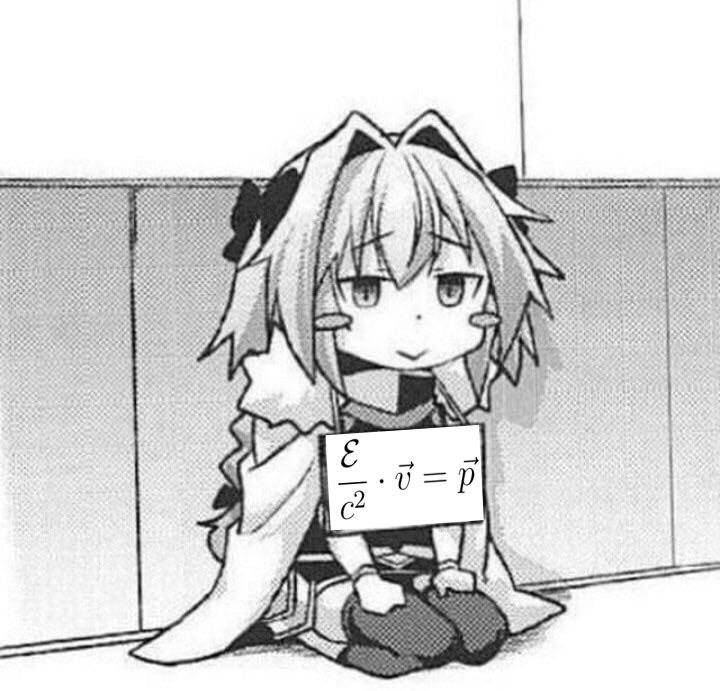
\includegraphics[width = 75mm]{figures/Astolfo_begging.jpg}
        }
    \end{figure*}
